\documentclass[border=4pt]{standalone}
% Shared typography and colours for the standalone figures.
\usepackage{unicode-math}
\setmainfont{TeX Gyre Termes}
\setmathfont{TeX Gyre Termes Math}
\usepackage{tikz}
\usetikzlibrary{arrows.meta,positioning,calc,decorations.pathreplacing}
\usepackage{pgfplots}
\pgfplotsset{compat=1.18}

% One colour per element or subsystem. Record the mapping in
% the working repository conventions and use it identically in every figure.
\definecolor{elemA}{HTML}{1F5FA8}
\definecolor{elemB}{HTML}{B8461B}
\definecolor{elemC}{HTML}{2E7D32}
\definecolor{elemD}{HTML}{6A4C93}
\definecolor{frameline}{HTML}{555555}

\begin{document}
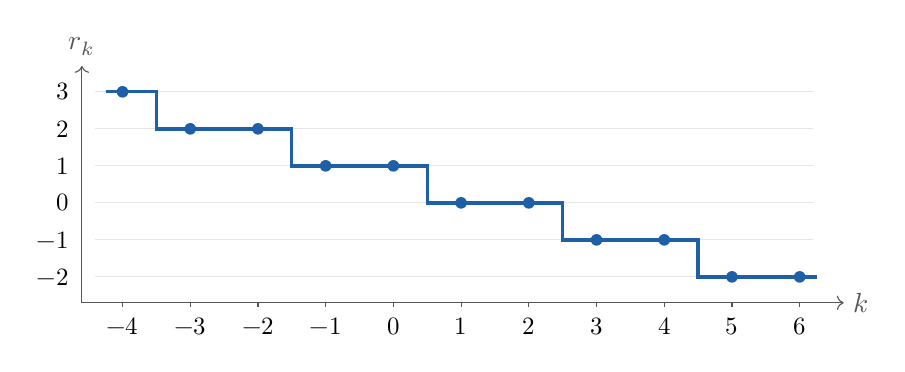
\begin{tikzpicture}[x=0.86cm,y=0.47cm]
  \draw[->,frameline] (-4.6,-2.7) -- (6.65,-2.7) node[right] {$k$};
  \draw[->,frameline] (-4.6,-2.7) -- (-4.6,3.7) node[above] {$r_k$};
  \foreach \k in {-4,-3,...,6} {
    \draw[frameline] (\k,-2.7) -- (\k,-2.82);
    \node[below,font=\small] at (\k,-2.84) {$\k$};
  }
  \foreach \r in {-2,-1,...,3} {
    \draw[frameline!15] (-4.4,\r) -- (6.2,\r);
    \node[left,font=\small] at (-4.65,\r) {$\r$};
  }
  \draw[elemA,very thick] (-4.25,3) -- (-3.5,3) -- (-3.5,2)
    -- (-1.5,2) -- (-1.5,1) -- (0.5,1) -- (0.5,0)
    -- (2.5,0) -- (2.5,-1) -- (4.5,-1) -- (4.5,-2) -- (6.25,-2);
  \foreach \k/\r in {-4/3,-3/2,-2/2,-1/1,0/1,1/0,2/0,3/-1,4/-1,5/-2,6/-2}
    \fill[elemA] (\k,\r) circle[radius=2.1pt];
\end{tikzpicture}
\end{document}
